\chapter{Classification}\label{Classification}
The classification task is a task of estimating the correct classes of objects. It has a wide appeal. For example,  classification is involved in detection tasks such as image recognition, medical diagnosis, speech analysis \& support, etc. Loan companies would like to predict the reliability of their customers in order to minimize the risk of impossible refunds. Another example is the detection of oil slicks from satellite images in order to give early warning of ecologic disasters and deter illegal dumping. 

One approach to the classification task is the one proposed in machine learning. Given data describing the relationship between the object space and class set, the approach is to train a classifier. The classifier is  the solution to the task: it estimating the correct classes of new objects.

This chapter considers in detail the machine-learning approach to the classification task. The task and the approach are formalized in section \ref{classification-task}. Section \ref{classifier-example} describes a typical learning algorithm (C4.5) as example. The classifier evaluation is provided in section \ref{classification-evaluation}. 




\section{Classification Task}\label{classification-task}
 
The classification task  is defined as follows~\cite{RegionClassif08}: assume an object space $X$ defined on $m$ features and a set $Y$ of possible classes. The instance space $Z$ over $X$ and $Y$ is defined as \(X \times Y\). The training data \(B\) is a bag \(\lbrace z_1,z_2,...,z_n \rbrace\) of instances \(z_i \in Z\) drawn from the same unknown probability distribution \(P_Z = P_{XY}\).  The classification task is to estimate the correct class of an object $x \in X$.

The machine learning approach to the classification task assumes the presence of   a fixed set \(H \subseteq Y^X\) of classifiers $h$ usually called hypothesis space.  Given the training data \(B\) we need to identify the best classifier in the hypothesis space H. For that purpose we employ a learning algorithm that searches the space H. The output of the algorithm is the desired classifier that can be used for classifying new objects.

The training data,  learning algorithm and  hypothesis space determine a set of assumptions that deductively imply for any object $x \in X$ the class assigned by the classifier to x. This set of assumtions is known as the inductive bias of the classifier. The inductive bias has to be chosen carefully so that the classifier is neither overfitted nor underfitted. The classifier is overfitted (underfitted) if there exists another classifier in the hypothesis that (1) performs better on most data derived from Z according to $P_Z$ and (2) performs worse (better) on the training data.

The learning process can be hindered by noise. There exist two types of noise. The first one is class noise, indicating that the class label of some of the training instances is incorrect. The second type is feature noise, indicating that  some feature values are incorrect of some of the instances. Feature noise can imply class noise or internal class noise. For short, we will use the term feature noise to indicate internal feature class noise.


\section{Example of a classifier: C4.5}\label{classifier-example}
An example of the machine learning approach to the classification problem is the well-known family of decision tree classifiers. These algorithms produce decision trees as classifiers, that are often robust to noisy data and capable of learning disjunctive expressions. Below, we illustrate their main idea through the example of C4.5, a possible approach to decision tree learning.

C4.5 employs a top-down, greedy search through the space of possible decision trees. It starts the construction of a decision tree by selecting a root node (representing a certain feature), and assigning different leaves based on possible feature values. The process is then iterated for each leaf until all training instances are correctly classified by the tree (or some stopping criteria are met). Figure~\ref{fig:dttennis} shows an example of a typical decision tree.

\begin{center}
\begin{figure}[h]
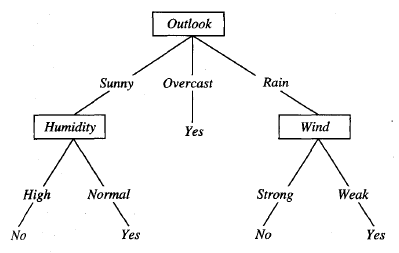
\includegraphics[scale=0.70]{img/ex_decisiontree.png}
\caption{A decision tree for the class \textit{PlayTennis} (which can take the values \textit{Yes} and \textit{No}). An example is classified by navigating through the tree to the appropriate leaf node, then returning the classification associated with this leaf. This tree classifies Saturday mornings according to whether they are suitable for playing tennis.}
\label{fig:dttennis}
\end{figure}
\end{center}

In order to select meaningful features, C4.5 measures how well a given feature separates the training examples according to their target classification. The measure it uses for this purpose is the \textit{Information Gain} measure. This measure is based on the entropy estimate, which characterizes the impurity of an arbitrary set of examples. The entropy of a sample $S$ is defined as follows:

\begin{center}$H(S) = - \sum_{i=1}^{|\mathbf{Y}|} \widehat{P}(y_i|S) \log_2 \widehat{P} (y_i|S)$\end{center}

where $\widehat{P}(y_i|S)$ is the estimated probability of examples in $S$ being labeled with class $i$. When $S$ has been partioned into $S_L$ and $S_R$ in a certain node, the weighted entropy of such a decision/split is defined as follows:

\begin{center}$H(S_L,S_R) = \frac{|S_L|}{|S|}H(S_L) + \frac{|S_R|}{|S|}H(S_R)$\end{center}

Notice entropy is 0 when all members of $X$ belong to the same class (the data is perfectly classified), and 1 if the data contains an equal proportion of positive and negative examples. Finally, the information gain for a given split then measures the expected reduction in entropy, and is defined as:

\begin{center}$Gain(S,S_L,S_R) = H(S) - H(S_L,S_R)$ \end{center}

The higher the Information Gain, the more reduction in entropy due to the split. Possible splits are evaluated and the one resulting into the highest gain is chosen. Therefore, selected trees place the features with highest information gain closest to the root. This process continues until all training examples are perfectly classified. To avoid overfitting (and to move more towards underfitting), two types of strategies can be implemented: pre-pruning and post-pruning. Pre-pruning implies that we do not allow the tree to grow completely, and stop the process in an earlier stage. Post-pruning implies that we completely grow the tree, and prune the tree afterwards.  

When the construction of a decision tree is finished, new objects can be classified. This is achieved by simply moving through the tree according to the object's feature values. The class label which is connected to the attained leaf node then represents the prediction for the class of the object.~\cite{MachineLearning97Mitchell}
 

\section{Evaluation}\label{classification-evaluation}

To decide whether to employ a   classifier we need to evaluate its classification performance. Below we consider the main  metrics for and approaches to
 classifier evaluation. 


\subsection{Evaluation Metrics}\label{eval-metrics}
Given a discrete classifier and a bag $D_t \subseteq Z$ of test instances,
we can construct a confusion matrix (see the first $|\mathbf{Y}|$ rows of the
matrix in Figure \ref{matrix:fig}). The matrix gives the counts of
the test instances depending on their true class and predicted
class provided by the classifier. We consider two types of counts:
\begin{itemize}

\item count $C_{ii}$ of true positive instances of the class $y_i \in \mathbf{Y}$ defined as instances of the class $y_i$ that
are correctly classified to belong to this class;

\item count $C_{ij}$ of false positive instances of the class $y_i \in \mathbf{Y}$ w.r.t.   the class $y_j \in \mathbf{Y}, y_i \neq y_j$ defined as instances of the class $y_j$ that are incorrectly classified to belong to the class $y_j$.
\end{itemize}

\begin{table}[h]
\centering                            % centering table
\begin{tabular}{|l| c| c c c c|}              % creating 10 columns
\hline                                % inserting double-line
& & \multicolumn{4}{|c|}{Actual} \\
\hline 
& & Class 1 & Class 2 & & Class $\mathbf{Y}$ \\ [0.5ex]
\hline                                      % inserts single-line
& Class 1 & $C_{11}$ & $C_{12}$ & \ldots & $C_{1|\mathbf{Y}|}$ \\
& Class 2  & $C_{21}$  &  $C_{22}$  & \ldots & $C_{2|\mathbf{Y}|}$ \\
\raisebox{1.5ex}{Predicted}  & & \raisebox{1.5ex}{\ldots} & \raisebox{1.5ex}{\ldots}  & & \raisebox{1.5ex}{\ldots} \\
& Class $\mathbf{Y}$ &  $C_{|\mathbf{Y}|1}$ & $C_{|\mathbf{Y}|2}$ & \ldots & $C_{|\mathbf{Y}||\mathbf{Y}|}$ \\
\hline                          % inserts single-line
\end{tabular}
\label{matrix:fig}
\end{table}

 
The counts from a confusion matrix are used for deriving useful metrics characterizing the performances of the classifier being evaluated. 

As an example, well-known metrics are accuracy rate $Ar$  and precision rate $Pr$  for class $y_i \in \mathbf{Y}$. They are
defined as follows:

\begin{eqnarray}
&&Ar = \frac{\sum_{i =1}^{|\mathbf{Y}|}C_{ii}}{\sum_{i =1}^{|\mathbf{Y}|}\sum_{k=1}^{|\mathbf{Y}|} C_{ik}} \label{a}\\
&&Pr_i = \frac{ C_{ii}}{\sum_{k=1}^{|\mathbf{Y}|} C_{ik}}  \label{p}
\end{eqnarray}

The most basic metrics are the true positive rate ({\it TPr}) of the class $y_i \in \mathbf{Y}$  and false positive rate ({\it FPr}) of the class $y_i \in \mathbf{Y}$ w.r.t. $y_j \in \mathbf{Y}, y_i \neq y_j$:


{\small
\[ TPr_i = \frac{C_{ii}}{\sum_{k=1}^{|\mathbf{Y}|} C_{ki}}\]
\[ FPr_{ij} = \frac{C_{ij}}{\sum_{k=1}^{|\mathbf{Y}|} C_{kj}}\]
}

 When the number of classes equals two, $TPr_1$ is also called sensitivity and $TPr_2$ specificity. Moreover, since the false positive rate in such case is only defined over one class, they are referred to as $FPr_1$ (the ratio of misclassifying class 1 as class 2) and $FPr_2$.

Another common metric to assess common performance over classifiers, is the area under the ROC curve. ROC curves are defined for 2-class classification problems (for simple, we call the first class the positive class, and the second class the negative class) and so-called scoring classifiers. Scoring classifiers are these classifiers that return for each instance to be classified a probability distribution. By default for 2-class problems,  if the probability of the first class is greater than 50\%, the first class is chosen. However, it is possible to choose any threshold between 0\% to 100\% to classify. Hence, we can define an infinite number of classifiers over one scoring classifier. So, a ROC curve of a scoring classifier is just the plot of the True Positive rate against the False Positive rate of all classifiers that can be achieved by changing the threshold. The idea behind this graph is that when a learner captures more instances of one class, it will generally misclassify more instances of the other class. Hence, ROC graphs depict the tradeoff between hit rates and false alarm rates of all possible classifiers. A ROC graph can be plotted by varying the probability threshold for predicting positive examples from 0 to 1. The advantage of this graph is that it shows for what region a classifier is superior compared to another. In order to come up with a single value that represents the expected performance of a ROC graph, one might measure the area under its curve, also called AUC. The AUC of a classifier is equivalent to the probability that the classifier will rank a randomly chosen positive instance higher than a randomly chosen negative instance. Thus, we should have classifiers with an AUC greater than 0.5 (which is equivalent to random guessing)~\cite{roc}~\cite{_miningwith}. 

\begin{figure}[h]
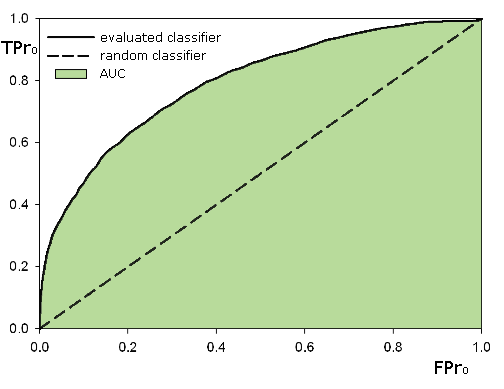
\includegraphics[scale=0.60]{img/roc-example.png}
\caption{An example of a ROC graph for class $0$ in a 2-class problem.}
\end{figure}


\subsection{Evaluation Approaches}
To evaluate classifiers we need a large independent test set. In many practical situations it is  impossible to obtain such an independent test set   since data labeling is very costly. Hence, the follwing evaluation approaches  have been proposed in order to overcome this problem. These approaches are briefly sketched below.

\paragraph{Holdout method and Random Subsampling}
In the holdout method, data is randomly partioned into two independent sets, namely a \textit{training} and a \textit{test} set. Typically, two-thirds of the data are allocated to the training set, and the remaining one-third is allocated to the test set. The training set is used to derive the model, after which the trained model is evaluated by comparing its predictions on the test set with their actual class labels. This estimate is however pessimistic, since only a portion of the initial data is used to derive the model.\\Random subsampling is a variation to the holdout method in which the holdout method is repeated \textit{k} times. The overall performance estimate is taken as the average of the performance measures obtained from each iteration.~\cite{Jiawei06}

\paragraph{Cross-validation}
In \textit{k}-fold cross-validation, the initial data are randomly partioned into \textit{k} mutually exclusive subsets (folds) each of approximately equal size. Training and testing is performed \textit{k} times. In iteration \textit{i}, fold \(D_i\) is reserved as the test set, and the remaining partitions are collectively used to train the model. Unlike the holdout and random subsampling methods, each sample is used the same number of times for training and once for testing. The overall performance is estimated by averaging the separate evaluations obtained during the \textit{k} iterations.\\Leave-one-out is a special case of \textit{k}-fold cross-validation where \textit{k} is set to the number of initial examples, such that each time only one sample is \textit{left out} at a time for the test set.

In stratified cross-validation, the folds are stratified so that the class distribution in each fold is approximately the same as that in the original dataset. In general, stratified 10-fold cross-validation is recommended for estimating classifier performance due to its relatively low bias and variance.~\cite{Jiawei06}


\subsection{Classifier Comparison}\label{classifcomp}
The metrics discussed in section~\ref{eval-metrics} allow one to compare the performance of several classifiers. However, in order to statistically prove that one classifier performs better than another, it is important that learning and evaluation is repeated several times using different training and test sets. As a result, each classifier will no longer be represented by one, but by a whole sample of values of the same performance measure. Usually, a \textit{paired t-test} is then used to compare such samples in order to calculate whether one classifier performs significantly better than another (according to the used evaluation metric). This calculation is based on the assumption that the obtained samples follow a Gaussian distribution. Thus, the paired t-test is used to compute whether the means of paired samples are equal, and therefore to prove whether one classifier produces better results than another.

\section{Conclusion}
It is clear that machine learning (ML) allows a wide variety of approaches to solve the classification task. Important to note is that no learning algorithm by definition is superior to others, but is able outperform them under specific conditions~\cite{supervised06}. Hence, the choice of any learning algorithm should be considered carefully. Preference for a certain classifier can be motivated by comparing its performance with others, as discussed in section~\ref{classification-evaluation}. However, it should be noted that restrictions regarding time or memory might hinder classifier implementation in some real-time applications.


